\chapter{\xlabel{pol2_dr_theory}POL-2 Data Reduction -- The Theory}
\label{sec:dr}
\section{\xlabel{dataflow}The Data Flow}

POL-2 data reduction is an involved process for which a broad overview
is first presented here before the specific details are discussed. It
is noted that this same procedure is used irrespective of whether a
single or multiple observations are to be reduced.

The data reduction process can be broken down into three main stages --
referred to as ``Run 1'', ``Run 2'' and ``Run 3'' in Figure~\ref{fig:pol2drflow}.

\begin{figure}[t!]
\begin{center}
\latexhtml{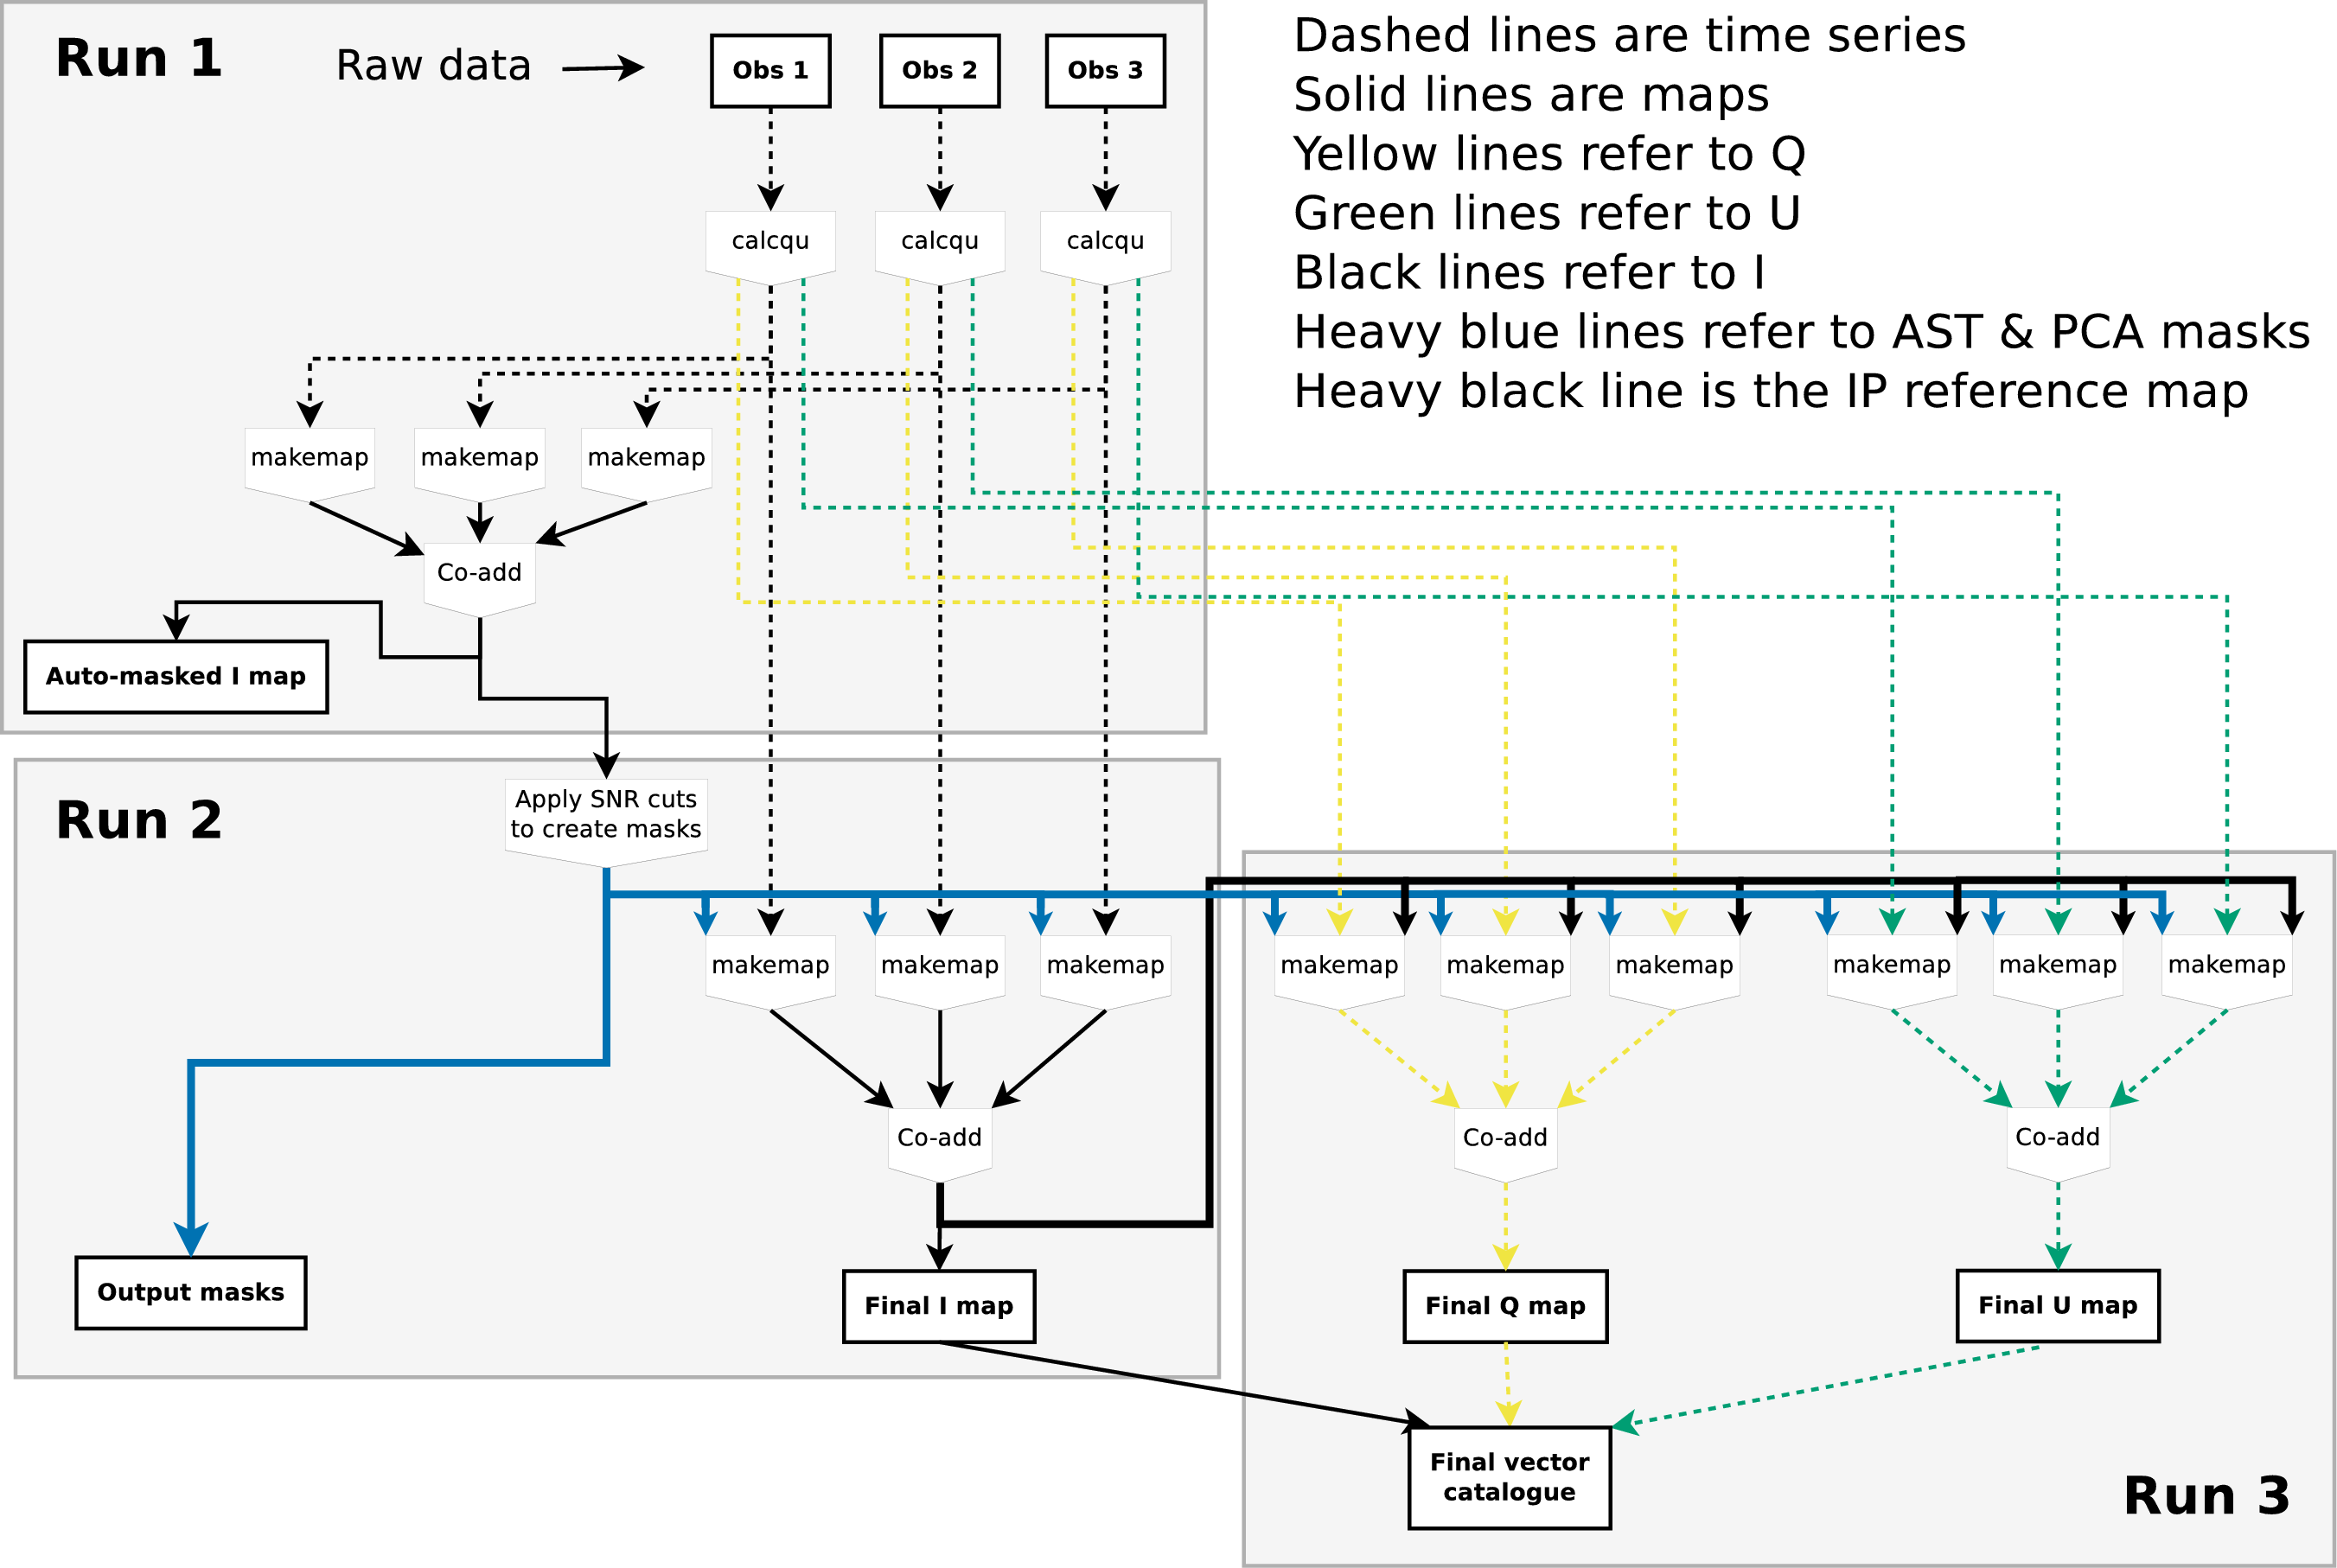
\includegraphics[width=1.25\linewidth,angle=90]{pol2map_flow}}{
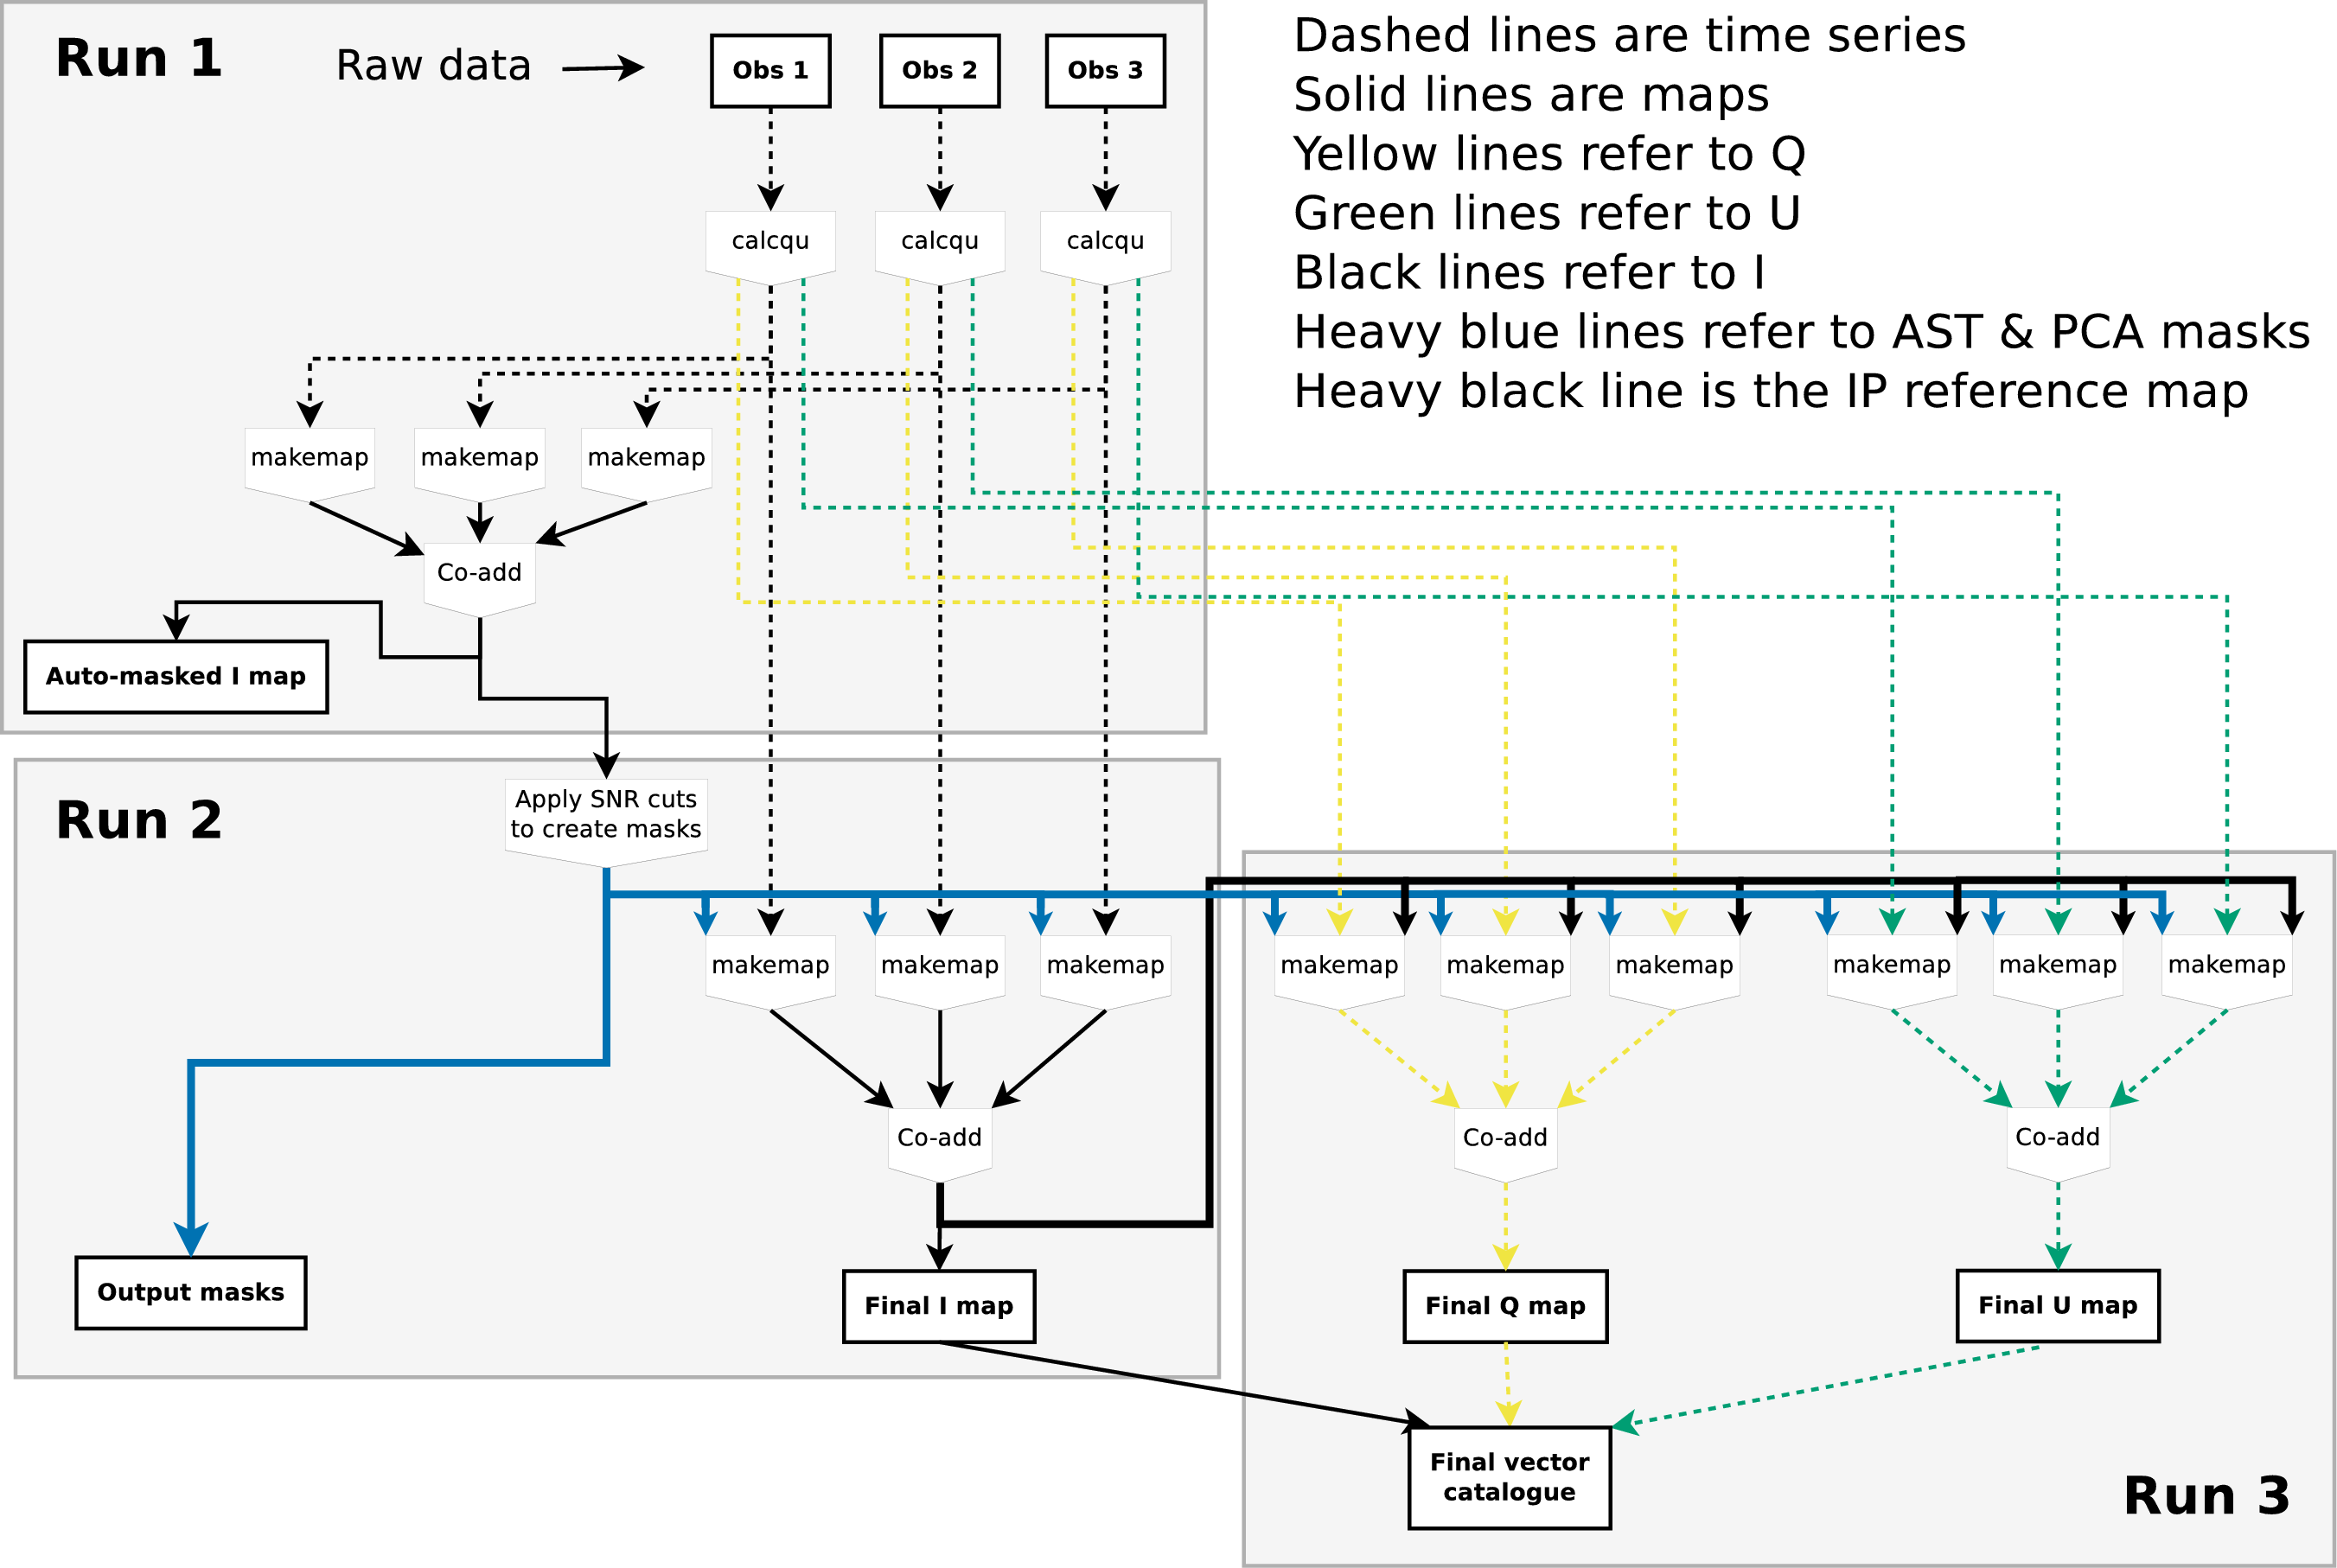
\includegraphics[width=1.0\linewidth]{pol2map_flow}}
\caption [POL-2 Data Flow]{ The data flow of the POL-2 data reduction
  method is presented. In this example, three POL-2 observations are
  reduced and combined in various stages and combination to produce I,
  Q and U maps and a vector catalogue.  }
\label{fig:pol2drflow}
\end{center}
\end{figure}


\subsection*{Step 1}

The initial step of the process (see Run~1 in Figure~\ref{fig:pol2drflow})
creates a preliminary co-added total intensity
(I) map from the raw data files for all observations provided to the
reduction routine (see \cref{Chapter}{sec:rundr}{}).


\subsubsection*{The process}
The analysed intensity values in the raw data time-streams are first
converted into Q, U and I time-streams using the
\xref{SMURF:\task{calcqu}}{sun258}{CALCQU} command (these are stored
for future use in the directory \texttt{qudata}, specified by the
\param{QUDIR} parameter in the example command below).

The \xref{SMURF:makemap}{sun258}{MAKEMAP} command is then used to
create a separate map from the I time-stream for each observation,
using SNR-based ``auto-masking'' to define the background regions that
are to be set to zero at the end of each iteration.

These maps are stored for future use in the directory \texttt{maps},
specified by the \param{MAPDIR} parameter. Each map has a name of the form:

\texttt{<UT$\_$DATE>$\_$<OBS$\_$NUM>$\_$<CHUNK$\_$NUM>$\_$imap.sdf}

where \texttt{<CHUNK$\_$NUM>} indicates the raw data file at the start
of the contiguous chunk of data used to create the map, and is usually
0003.  Each of these maps is compared to the specified reference map
(if any) to determine a pointing correction to be applied to the
observation in future. If no reference map is supplied, the I map
created from the first observation defines the expected source
position, and is compared with later maps to determine their pointing
corrections.

This step uses a PCA threshold of 50 (see Section~\ref{sec:pca} for more details).

\texttt{pca.pcathresh = -50}



\subsection*{Step 2}

In the second step of the process (see Run~2 in
Figure~\ref{fig:pol2drflow}) an improved I map is produced. These
improvements come from
\begin{enumerate}
\item applied relative pointing corrections
\item the use of an increased number of PCA components
  (\texttt{pca.pcathresh=-150})
\item using a single fixed mask for all observations. The mask is
  determined from the preliminary co-add I map and thus includes
  fainter structure than would be used if the mask was based on only
  one observation.
\end{enumerate}

\subsection*{Step 3}

In the third step of the reduction process (see Run~3 in
Figure~\ref{fig:pol2drflow}), both the Q and U maps are produced. The production
of the Q and U maps requires the Q and U time-series data (produced in
Step~1), the final I map (produced in Step~2) and the output masks (also
produced in Step~2). Once the Q and U maps are produced a final vector
catalogue is created.

\section{\xlabel{makemap}MAKEMAP}

The POL-2 data reduction builds upon the existing SCUBA-2 Dynamic
Iterative Map-Maker, hereafter just referred to as the map-maker. This
is the tool used to produce SCUBA-2 maps, and is invoked by the
\SMURF\ \makemap\ command. It performs some
pre-processing steps to clean the data, solves for multiple signal
components using an iterative algorithm, and bins the resulting
time-series data to produce a final science map.

In \poltwomap\ the map-maker is used in conjunction with
\xref{calcqu}{sun258}{CALCQU} (see
Section~\ref{sec:calcqu}) to produce maps of Q and U, as well as I.

\section{\xlabel{calcqu}CALCQU}
\label{sec:calcqu}

In addition to the POL-2 data reduction building on the
existing SCUBA-2 map-maker, \poltwomap\ also relies on the \SMURF\
command \task{CALQU}.

This \xref{calcqu}{sun258}{CALCQU} tool creates time series holding Q and U values from a set of POL-2
time series holding raw data values. The supplied time-series data files are first
flat-fielded, cleaned and concatenated, before being used to create
the Q and U values. The Q and U time-series are down-sampled to 2Hz
(\emph{i.e.} they contain two Q or U samples per second), and are 
chosen to minimise the sum of the squared residuals between the measured 
raw data values and the expected values given by Equation~\ref{eqn:idet}.


\section{\xlabel{pca}PCA}
\label{sec:pca}

One difference between the reduction of SCUBA-2 data and POL-2 data is the
method used to remove the sky background.  The sky background is usually
very large compared with the astronomical signal, and both are subject to
the same form of instrumental polarisation (IP -- see Section~\ref{sec:ip}).
This
IP acting on the high sky background values causes high background values
in the Q and U maps. However, there is evidence that the IP is not
constant across the focal plane, resulting in spatial variations in the
background of the Q and U maps.

For non-POL-2 data, the background is removing using a simple common-mode
model, in which the mean of the bolometer values is found at each time
slice and is then removed from the individual bolometer values. This
ignores any spatial variations in the background and so fails to remove
the background properly in POL-2 Q and U maps.

To fix this, a second stage of background removal is used when processing
POL-2 data, following the initial common-mode removal. This second stage
is based upon a Principal Component Analysis (PCA) of the 1280
time-streams in each sub-array (the Q and U data are processed
separately). The PCA process identifies the strongest time-dependent
components that are present within multiple bolometers. These components
are assumed to represent the spatially varying background signal and are
removed, leaving just the astronomical signal. The number of components
to remove can be specified by the user, via a \task{makemap} configuration
parameter called \xparam{PCA.PCATHRESH}{pca.pcathresh} although \poltwomap,
the reduction command for POL-2
data, provides suitable defaults for this parameter.

\begin{itemize}
\item first stage uses \param{pca.pcathresh} = -50
\item second stage uses \param{pca.pcathresh} = -150
\end{itemize}

On each \task{makemap} iteration, the PCA process removes the background (thus
reducing the noise in the map) but also removes some of the astronomical
signal. The amount of astronomical signal removed will be greater for
larger values of \texttt{pca.pcathresh}. However, this astronomical
signal is still present in the original time-series data and so can be
recovered if sufficient \task{makemap} iterations are performed. In other words,
using larger values of \param{pca.pcathresh} slows down the rate at
which astronomical signal is transferred from the time-series data to the
map, thus increasing the number of iterations required to recover the
full astronomical signal in the map.

Spatial variations in the sky background may also be present in non-POL-2
data, but at a lower level. For a discussion of why PCA is not routinely
run on non-polarimetric SCUBA-2 data, see \cref{Appendix}{app:pca}{}.



\section{\xlabel{masking}Masking}
A mask is a two-dimensional array which has the same shape and size as
the final map, and which is used to indicate where the source is
expected to fall within the map. `Bad' pixel values within a mask
indicate background pixels, and `good' pixel values indicate source
pixels. Masks are used for two main purposes.

\begin{enumerate}
\item They prevent the growth of gradients and other artificial large
  scale structures within the map.  For this purpose, the astronomical
  signal at all background pixels defined by the mask is forced to
  zero at the end of each iteration within \makemap\ (except for the
  final iteration).
\item They prevent bright sources polluting the evaluation of the
  various noise models (PCA, COM, FLT) used within \task{makemap}. Source
  pixels are excluded from the calculation of these models.
\end{enumerate}


The \poltwomap\ script uses different masks for these two purposes -- the
``AST'' mask and the ``PCA'' mask.  The PCA mask is in general less
extensive than the AST mask, with the source areas being restricted to
the brighter inner regions.  Each of these two masks can either be
generated automatically within \task{pol2map}, or be specified by a fixed
external NDF.



\section{\xlabel{tailoredDR}Tailoring a reduction}

\subsection*{Variances between POL-2 maps}

\param{MAPVAR} is a \poltwomap\ parameter that controls how the variances in the
coadded I, Q and U maps are formed.

If MAPVAR is set TRUE, the variances in the coadded I, Q and U maps
are formed from the spread of pixel data values between the individual
observation maps. If MAPVAR is FALSE (the default), the variances in
the coadded maps are formed by propagating the pixel variance values
created by \makemap\ from the individual observation maps (these are
based on the spread of I, Q or U values that fall in each pixel).

Use MAPVAR=TRUE only if enough observations are available to make the
variances between them meaningful.A general lower limit on its value
is difficult to define, but is advised a minimum of 10 observations.


If a test of the effect of this option is required on a field for which
the I, Q and U maps from a set of individual observations are already
available, the following may be done:

\begin{terminalv}
% pol2map in=maps/\* iout=imapvar qout=qmapvar uout=umapvar mapvar=yes \
                   ipcor=no cat=cat_mapvar debias=yes
\end{terminalv}

assuming that the I, Q and U maps are in directory \file{maps}. The
variances in \file{imapvar.sdf}, \file{qmapvar.sdf} and
\file{umapvar.sdf} will be calculated using the new method, and
these variances will then be used to form the errors in the
\file{cat$\_$mapvar.FIT} catalogue.



